%%%%%%%%%%%%%%%%%%%%%%%%%%%%%%%%%%%%%%%%%%%%%%%%%
% Trabalho de Conclus�o de Curso
% Aluno: Mario Henrique A. C. Adaniya
% Orientador: Prof. Dr. Mario Lemos Proen�a Jr.
% 
% Estrutura Principal
%%%%%%%%%%%%%%%%%%%%%%%%%%%%%%%%%%%%%%%%%%%%%%%%%
 
\documentclass[12pt,a4paper]{abnt}
%\usepackage[utf8]{inputenc}
\usepackage[latin1]{inputenc}
\usepackage[brazil]{babel}

\usepackage[pdftex]{graphicx}

\usepackage{latexsym} 
\usepackage{ae}
\usepackage{hyperref}
\usepackage[alf]{abntcite}
\usepackage{tabela-simbolos} %utilizado apenas para manter compatibilidade de codigo
\usepackage{longtable} % tabelas longas, utilizado na lista de simbolos
\usepackage{listings} % pacote para algoritmos
\usepackage{float}      
\usepackage{fancyvrb}
\usepackage{booktabs}
 
%\usepackage{chngcntr} %pacote para alterar contadores 
 
%===== C�digos Fonte =====
\newenvironment{codeverbatim}{\VerbatimEnvironment \small
   \begin{Verbatim}[xleftmargin=20mm]}
   {\end{Verbatim}}
%=======
\floatstyle{plain}  % tipos: plain, boxed, ruled
\newfloat{codigo}{tbp}{lop}[section]  % numera os captions com  n�mero de se��o.
\floatname{codigo}{C�digo}
% nome para ser usado no sum�rio
\newcommand{\listofcodename}{Lista de Codigos}
%=========================

\begin{document}

%	%%%%%%%%%%%%%%%%%%%%%%%%%%%%%%%%%%%%%
%% Capa
%%%%%%%%%%%%%%%%%%%%%%%%%%%%%%%%%%%%%

\thispagestyle{empty}

\begin{figure}[htb]
	\begin{center}
		%\begin{minipage}[b]{0.2\linewidth}
			%\begin{center}
				
\includegraphics[scale=0.9]{./figuras/uellogo1.jpg}
			%\end{center}
		%\end{minipage}
	%	\begin{minipage}[b]{0.7\linewidth}
			%	{\large \bf Universidade Estadual de Londrina\\[5pt]
				%		Centro de Ci�ncias Exatas\\[5pt]
						%				Departamento de Computa��o}
	%	\end{minipage}
	\end{center}
\end{figure}


\begin{center}
	Trabalho de Conclus\~{a}o de Curso

	{\autorformat M\'{a}rio Henrique A. C. Adaniya}
\end{center}

\vspace*{\stretch{3}}

\begin{center}
{\tituloformat T�cnicas de Extra��o de Informa��es da Web}
\end{center}

\vspace*{\stretch{3}}

\vspace*{\stretch{4}}

\begin{center}
{\bf Londrina \\
2009}
\end{center}

%	%%%%%%%%%%%%%%%%%%%%%%%%%%%%%%%%%%%%%
%%   Folha de rosto
%%%%%%%%%%%%%%%%%%%%%%%%%%%%%%%%%%%%%

\autor{M�rio Henrique A. C. Adaniya}
\titulo{T�cnicas de Extra��o de Informa��es da Web}
\orientador[Orientador:]{Mario Lemos Proen�a Jr.}
\comentario{Trabalho apresentado �  Universidade Estadual de Londrina, como parte do requisito para obten��o do t�tulo de Bacharel em Ci�ncia da Computa��o, sob orienta��o da Prof\textord Doutor \\Mario Lemos Proen�a Jr.}
\instituicao{Universidade Estadual de Londrina}
\local{Londrina}
\data{2009}

	 
	\sumario \label{sumario}
%	\addcontentsline{toc}{chapter}{\listofcodename}
%	\listoftables
%	\listadesiglas
%	\listof{codigo}{\listofcodename}  % Lista de C�digos 
   
    \chapter{Introdu��o} \label{INTRO}

		Os avan�os inimagin�veis presenciados atualmente, ajudam para uma globaliza��o e moderniza��o do mundo como nunca poderiamos prever. As informa��es e como elas s�o tratadas tamb�m sofreram dr�sticas altera��es, e podemos destacar como um grande fator o advento da \textit{Internet}. Atualmente � improv�vel nos imaginarmos sem a \textit{Internet} e suas facilidades. Alguns acreditam que a import�ncia da \textit{Internet} em nossas vidas num futuro pr�ximo ser� tratada como a necessidade da energia el�trica, �gua e saneamento b�sico, entre outros servi�os que tomamos como essenciais hoje \cite{Proenca2005}. Empresas t�m preju�zos na casa dos bilh�es por algumas horas sem \textit{Internet}, tal qual, sua import�ncia hoje.
	
		Cada vez mais encontramos toda e qualquer informa��o que precisamos dispon�veis \textit{online}. � uma tend�ncia que grandes editoras com revistas e publica��es impressas est�o aderindo, mantendo os impressos tradicionais e publicando virtualmente os mesmos conte�dos e adicionando outros exclusivos na edi��o \textit{online}. A \textit{World Wide Web (Web)} � um meio de comunica��o popular e interativo para disseminar informa��o atualmente \cite{Kosala2000}. Todo dia, mais e mais p�ginas s�o indexadas pelos motores de buscas. \textit{Blogs} surgem aos milhares com pessoas expressando suas id�ias, opini�es e experi�ncias. Sites de relacionamento, f�runs, \textit{Wikis} armazenam conte�dos imensos dos mais diversificados assuntos. E neste pandem�nio, como encontrar o que estamos procurando? Como descobrir se a informa��o recuperada � confiavel? 
	
		A area da Extra��o da Informa��o(EI) possui como meta localizar informa��es relevantes em documentos ou um conjunto de documentos expresso em lingua natural, extra�-las e estrutura-l�s, por exemplo, em banco de dados a fim de facilitar sua manipula��o e an�lise \cite{Alvarez2007}.
	
		A Minera��o na \textit{WEB(Web Mining)} envolve in�meras disciplinas como Recupera��o da Informa��o, Extra��o da Informa��o, Estat�stica, Intelig�ncia Artificial e Minera��o de Dados, entre muitas outras \cite{Alvarez2007}.		
	
		Atualmente, como o acesso a \emph{Internet} � muito mais f�cil, e tamb�m � a publica��o de qualquer conte�do por qualquer pessoa, a busca por uma informa��o concreta de uma fonte segura torna-se importante. Para tal, � necess�rio buscar formas de pesquisa mais interessantes adicionais as pesquisas j� exitentes.
		
		A busca pela informa��o correta se torna um assunto muito mais s�rio quando se trata de sa�de, pois com o acesso facilitado, muitas pessoas ao primeiro sintoma de alguma doen�a buscam informa��o na \emph{Internet} e t�o logo, podem ter acesso a informa��es, tanto corretas quanto incompletas ou na pior das hip�tese, informa��es erradas. A pessoa pode seguir conselhos equivocados e n�o procurar assist�ncia m�dica, podendo agravar sua situa��o.
		
		Por outro lado, gra�as aos estudos em minera��o de dados na \emph{Web} temos alguns sites de \emph{E-Commerce} muito mais personalizados. Como grandes exemplos temos o Submarino\footnote{Submarino - http://www.submarino.com.br} e Lojas Americanas\footnote{Lojas Americanas - http://www.lojasamericanas.com.br}, no mercado nacional. Podemos perceber isto quando efetuamos uma compra de algum livro pelo Submarino, e nas visitas posteriores ao site, ele nos indica g�neros literarios semelhantes ao livro comprado. E cada vez mais este tipo de mecanismos s�o utilizados em muitas outras �reas.
	
	\section{Organiza��o do Trabalho}

	O assunto abordado no trabalho, se dar� da seguinte maneira:

	No cap�tulo~\ref{RI} s�o vistos alguns conceitos sobre Recupera��o de Informa��o. A preocupa��o principal desta area sempre foi encontrar maneiras eficazes de selecionar documentos. Importante ressaltar que a informa��o contida n�o possui destaque na recupera��o. A informa��o ganha uma conota��o importante no cap�tulo~\ref{EI}, onde s�o abordados os conceitos sobre Extra��o de Informa��o. Com alguns destes conceitos fundamentados, analisamos a Minera��o de Dados na Web no cap�tulo~\ref{WebMining}.
	
	Por fim, fazemos uma conclus�o sobre o trabalho at� o momento, e futuros conte�dos que ser�o estudados e abordados numa vers�o final do trabalho.
	\chapter{Recupera��o de Informa��o} \label{RI}

		Recupera��o de Informa��o (RI) � a tarefa de encontrar documentos relevantes a partir de um \textit{corpus} ou conjunto de textos em resposta a uma necessidade de informa��o de um usu�rio \cite{Smeaton1997}. Um dos maiores problemas enfrentados desde seu in�cio, e que perpetua atualmente � a informa��o estar contida em linguagem natural. Quando a \emph{WWW} foi concebida, a comunidade acad�mica que tratava de RI concentraram suas aten��es para uma melhoria dos motores de busca, voltando a impulsionar o crescimento da RI.
				 		
		RI possui limites bem delimitados, e qualquer tarefa al�m de prover ao usu�rio os documentos, n�o � um sistema de recupera��o de informa��o. A tecnologia de RI � quase sempre encontrada no n�cleo de funcionalidades dos sistemas de busca de informa��es de uma maneira impercept�vel para o usu�rio. T�cnicas como: filtragem, roteamento, categoriza��o e clusteriza��o  possuem em comum a busca e compara��o dos documentos e as necessidades do usu�rio \cite{Smeaton1997}.
		
		\begin{itemize}
		  \item filtragem - atrav�s do fluxo de documentos entre um certo perfil ou grupo de usu�rios, refletindo a informa��o desejada;
		  \item categoriza��o - � a tarefa de categorizar o documento em um conjunto pr�-definido de categorias;
		  \item roteamento - divide a entrada de documentos para grupos ou usu�rios baseado no conte�do;
		  \item clusteriza��o - � o agrupamento de documentos semelhantes para posterior busca ou outra utiliza��o;
		\end{itemize}		
				
		%Resumidamente a opera��o de um sistema de RI ocorre com o usu�rio descrevendo suas necessidades para o sistema, ent�o o sistema retorna os documentos que correspondem. Smeaton \cite{Smeaton1997} sugere algumas m�tricas heur�sticas\footnote{Os estudos abordados quanto aos modelos matem�ticos descritos pelo autor foram no �mbito superficial.} para tal ordenamento  e enumera �reas onde a pesquisa de RI s�o bem ativas.
		
%		A opera��o de recupera��o em sistemas de RI objetiva computar graus de coincid�ncia entre a consulta do usu�rio e os documentos para ordenar cada documento. Smeaton \cite{Smeaton1997} sugere algumas m�tricas heur�sticas para tal ordenamento  e enumera �reas onde a pesquisa de RI s�o bem ativas tais como a recupera��o baseada em \emph{clusters}, a recupera��o pela combina��o de diversas estrat�gias, indexa��o sem�ntica latente, recupera��o de passagem e documentos de comprimento heterog�neo.
				
		Sistemas de RI s�o estruturados atrav�s da defini��o da fonte de informa��o com a qual se trabalha, ou seja, os tipos de documentos que ser�o indexados. Posteriormente, as opera��es que ser�o executadas no momento das buscas devem ser determinadas, estruturando os documentos de acordo com as tarefas a serem executadas. Em seguida, um �ndice com os termos contidos nos documentos � criado \cite{Baeza-Yates1999}. Com uma consulta, o usu�rio descreve suas necessidades atrav�s de termos e o processo de RI � iniciado \cite{Beppler2008}.
		
		A opera��o de recupera��o em sistemas de RI objetiva computar graus de coincid�ncia entre a consulta do usu�rio e os documentos para ordenar cada documento. Smeaton \cite{Smeaton1997} sugere algumas m�tricas heur�sticas para tal ordenamento  e enumera �reas onde a pesquisa de RI s�o bem ativas. 
		
		O problema da aquisi��o de conhecimento de textos v�m sendo questionado pela comunidade de RI em fun��o da r�pida pulveriza��o de informa��o impulsionada pela \emph{Internet}. A pesquisa sobre atividades baseadas em \emph{corpus} de textos t�m sido encorajada, facilitando o desenvolvimento de solu��es.
		
%		Motivado pela forte interdepend�ncia entre a RI e o processamento de linguagem natural, Smeaton (1995, 1995a, 1995b) questiona a real utilidade do processamento de linguagem e dos demais recursos ling��sticos para a RI. O autor alega que o processamento de linguagem natural oferece um aux�lio modesto para a efici�ncia da RI pelo fato das t�cnicas de processamento de LN terem sido desenvolvidas visando aplica��es de tradu��o autom�tica e interfaces de linguagem natural. Uma caracter�stica que limita a ajuda oferecida pelas t�cnicas de processamento de LN oriunda-se na complexidade destas t�cnicas tornando-as eficientes apenas quando aplicadas sobre uma pequena quantidade de textos. Uma solu��o para este problema � proposta em Zhai (1997) que apresenta um m�todo para indexa��o de documentos testado num conjunto de documentos de 250 mega bytes. Neste m�todo, o autor prop�e um modelo probabil�stico para realizar um parsing de express�es ao inv�s da indexa��o por palavras, demonstrando uma significativa melhora na recupera��o.

%		Outras t�cnicas al�m das baseadas em linguagem natural tamb�m podem beneficiar a tecnologia de RI. O m�todo relevance feedback (Haines e Croft, 1993) aprimora a qualidade da recupera��o de informa��o inteligente ao modificar a consulta baseando-se na retroalimenta��o do usu�rio. A consulta � modificada atrav�s de uma modifica��o nos pesos que caracterizam seus termos motivada pela informa��o dada pelo usu�rio. O m�todo relevance feedback � proposto em Haines e Croft (1993) como um aprimoramento do modelo de recupera��o que utiliza Redes de Infer�ncia (Turtle, 1991). Redes de infer�ncia s�o um modelo de recupera��o de informa��o baseado em probabilidade para racioc�nio com incerteza. A rede de infer�ncia � um grafo com quatro tipos diferentes de n�s: para documentos, para a representa��o conceitual do conte�do dos documentos, para as consultas, e o �ltimo para a informa��o desconhecida. A cada nova consulta, os n�s s�o instanciados para cada documento do conjunto e as probabilidades s�o propagadas para inferir uma probabilidade associada � informa��o desconhecida; gerando, assim, um ordenamento dos documentos.

%		Uma aplica��o do m�todo de redes de infer�ncia na recupera��o de informa��o � o sistema de recupera��o (Callan, Croft, e Harding, 1992) que vem sendo implementado com sucesso sobre uma base de 1 giga byte. O sistema INQUERY cont�m um subsistema de parsing que comporta uma indexa��o sofisticada e uma complexa formula��o nas consultas.

%		O m�todo de relevance feedback do sistema INQUERY foi utilizado por Daniels & Rissland (1995) em uma pesquisa que tamb�m ressalta a import�ncia do uso do paradigma de RBC na recupera��o da informa��o. As autoras prop�em um sistema h�brido de RBC-RI que realiza a busca por documentos similares em uma pequena base de conhecimento de casos em fun��o das fortes necessidades de representa��o de conhecimento que ofereceria uma base maior. O resultado gerado pelo sistema baseado em casos � um conjunto de textos que sugerem uma lista de termos que � usada para definir uma consulta que conduz a recupera��o de documentos baseada em textos.
  
  	\section{Modelos de Recupera��o de Informa��o}\label{RI:Modelos}
  	
%  		De acordo com Baeza-Yates e Ribeiro-Neto \cite{Baeza-Yates1999}, podemos decompor um modelo de RI em \cite{Beppler2008}:
%  		\begin{itemize}
%  		  \item um conjunto de vis�es l�gicas de documentos de uma cole��o - � a forma como o documento � indexado, e.g., palavras-chaves;
%  		  \item um conjunto de vis�es l�gicas da informa��o prestada pelo usu�rio;
%  		  \item um framework para modelar documentos, consultas e suas rela��es - tecnologia utilizada para prover as ;
%  		  \item uma fun��o de ordena��o - fun��o de ordena��o escolhida para retornar os resultados.
%  		\end{itemize}
  		
  		Greengrass \cite{Greengrass2000} prop�em duas categorias para os modelos de RI: sem�nticos e est�tisticos. Os sem�nticos tem a preocupa��o de ``entender'' um texto em linguagem natural. Quanto aos modelos est�tisticos, s�o atribuidos medidas estat�sticas mensurando a compara��o entre uma consulta e um documento. Na categoria est�tistica enquandramos os modelos: Booleano, Booleano Estendido, Vetorial, Probabil�stico, Difuso e Indexa��o Sem�ntica Latente. O modelo de Processamento de Linguagem Natural representa a categoria sem�ntica. 
  	
  	\subsection{Modelo Booleano}
  	  		
  		Utilizando-se da teoria dos conjuntos e �lgebra booleana, as consultas s�o construidas atrav�s de express�es booleanas e conectores l�gicos: AND, OR, NOT. A recupera��o de um determinado documento s� � efetuada mediante um valor verdadeiro das express�es, no nosso caso, uma consulta. Devido a simplicidade e ao formalismo, temos um resultado n�o ordenado, acarretando tamb�m � recupera��o de muitos ou poucos documentos \cite{Baeza-Yates1999}.
  		
  	\subsection{Modelo Booleano Estendido}
  	
  		Este modelo � proposto com algumas melhorias em rela��o seu predescessor, implementando uma fun��o de ordena��o e a utiliza��o de diferentes operadores. Este modelo atribui valores no intervalo $[0,1]$, que equivale ao grau de compara��o de uma express�o com um documento \cite{Lee1994}.
  	
  	\subsection{Modelo Vetorial}
  	
  		Este modelo � representado por um vetor ou uma lista de termos ordenados. O grau de similaridade de um documento em rela��o a uma consulta � a avalia��o entre os vetores que representam o documento e a consulta. Com isto, uma ordena��o de acordo com o grau de similaridade � executada dada uma consulta \cite{Baeza-Yates1999}.
  		
  	\subsection{Modelo Probabil�stico}
  	
  		Fazendo-se uso de c�lculos probabil�sticos, o modelo calcula a probabilidade condicional em que um determinado documento � relevante a uma dada consulta. Consulta e documentos s�o representados por meio de um conjunto de termos, calculando-se a probabilidade de ocorr�ncia dos termos de uma consulta em documentos relevante e n�o-relevantes. A fun��o probabilistica depende do modelo a ser usado, bem como os termos est�o distribuidos entre os documentos \cite{Greengrass2000}.
  		
	\subsection{Modelo Difuso}
	
		� um modelo extendido do modelo booleano e possui uma fun��o de ordena��o cujo resultado da compara��o entre um documento e uma consulta � aproximado. Como Zadeh redefiniu o intervalo fechado do conceito cl�ssico da pertin�ncia de $[0,1]\in\mathbb{Z}$ para o intervalo cont�nuo $[0,1]\in\mathbb{R}$ \cite{Baeza-Yates1999}. 
		
		A aproxima��o considera que cada termo de uma consulta define um conjunto difuso e cada documento possui um grau de participa��o nesse conjunto. Muitas cr�ticas s�o lan�adas a este modelo por gerar medidas incorretas \cite{Lee1994}.
		
		A principal justificativa para o m�todo difuso � a falta de informa��o frequente do usu�rio e do pr�prio sistema em saber se o documento possui a informa��o consultada ou n�o \cite{Lee1994}.

	\subsection{Modelo de Indexa��o Sem�ntica Latente}
	
		A indexa��o sem�ntica latente (LSI) � uma t�cnica autom�tica que analisa as co-ocor�ncias de termos em documentos textuais almejando descobrir relacionamentos entre eles.
		
		LSI � um modelo que consome processamento devido as estruturas escolhidas para a analise dos textos, no caso, uma matriz esparsa termo-documento. Utilizando a Decomposi��o de Valores Singulares (SVD), a matriz � decomposta em outras tr�s matrizes. 
		
		Este � um modelo que visa a captura de termos e suas depend�ncias que podem ter um significado sem�ntico.
		  	
  	\subsection{Modelo de Processamento de Linguagem Natural}
  	
  		O modelo que usa processamento em linguagem natural pode ser categorizado como modelo sem�ntico, porque a estrutura e o significado dos documentos est�o intimamente ligados ao modelo. Raramente s�o utilizadas em RI, mas geralmente s�o empregadas em conjunto com outros modelos estat�sticos \cite{Greengrass2000}.
  		
  		Smeaton \cite{Smeaton1997} defende que as t�cnicas de processamento de linguagem natural adotadas na RI apenas auxiliam eficientemente quando utilizadas em pequenas quantidades de textos. Assim sendo, a complexidade de t�cnicas de PLN � oriunda das aplica��es para a qual fora desenvolvida como tradu��o autom�tica e interfaces de linguagem natural.
  		 
  		%Motivado pela forte interdepend�ncia entre a RI e o processamento de linguagem natural, Smeaton (1995, 1995a, 1995b) questiona a real utilidade do processamento de linguagem e dos demais recursos ling��sticos para a RI. O autor alega que o processamento de linguagem natural oferece um aux�lio modesto para a efici�ncia da RI pelo fato das t�cnicas de processamento de LN terem sido desenvolvidas visando aplica��es de tradu��o autom�tica e interfaces de linguagem natural. Uma caracter�stica que limita a ajuda oferecida pelas t�cnicas de processamento de LN oriunda-se na complexidade destas t�cnicas tornando-as eficientes apenas quando aplicadas sobre uma pequena quantidade de textos. Uma solu��o para este problema � proposta em Zhai (1997) que apresenta um m�todo para indexa��o de documentos testado num conjunto de documentos de 250 mega bytes. Neste m�todo, o autor prop�e um modelo probabil�stico para realizar um parsing de express�es ao inv�s da indexa��o por palavras, demonstrando uma significativa melhora na recupera��o.
  		
  	
  	\section{Recupera��o de Informa��o na WEB}\label{RI:webRI}			

		Quando estamos lidando com a \emph{Web} temos um cen�rio que contrasta com a chamada RI Cl�ssica. Na RI Cl�ssica temos um dom�nio e usu�rios definidos, quando na \emph{Web} encontramos um cen�rio din�mico e usu�rios consultando simultaneamente as informa��es \cite{Kobayashi1999}. 
		
		Muitas caracter�sticas devem ser levadas em conta quando estamos recuperando documentos na \emph{WEB} \cite{Huang2000}:
		
		\begin{itemize}
          \item \textbf{Tamanho da Internet} - O tamanho da \emph{Internet}, segundo Zhang e seu grupo de pesquisa \cite{Zhang2008}, estima-se que em Janeiro de 2008 a Internet continha 62400000 hostnames ativos. De acordo com a pesquisa, a Lei de Moore\footnote{A Lei de Moore foi predita por um dos fundadores da Intel, Gordon Moore, e sugere que a cada dezoito meses a capacidade de transitores no CPU dobra. Apareceu em 1965 e se manteve como verdade por quase meio s�culo, e costuma ser utilizada para prever modelos futuros de tecnologias.} � observada, exceto que para a Internet, foi visto que a cada cinco anos, ela dobra de tamanho. Importante esclarecer que os dados do tamanho da \emph{Internet} v�ria de acordo com grupos de pesquisa, mas todos chegam a resultados similares quanto ao crescimento exponencial;
          \item \textbf{Dinamismo da Internet} - As t�cnicas de Recupera��o de Informa��o s�o geralmenta est�tica, enquanto a \emph{Web} est� em constante metamorfose;
          \item \textbf{Duplica��o} - 30\% do cont�udo da \emph{Internet} � uma c�pia de algum conte�do existente;
          \item \textbf{Comportamentos espec�ficos} - � estimado que 85\% dos usu�rios utilizam apenas a primeira p�gina retornada das \emph{search engines}, e 28\% modificam sua consulta original;
          \item \textbf{Multiplos tipos de usu�rio} - Possui muitos tipos de usu�rios e cada usu�rio utiliza a \emph{Internet} para uma tarefa espec�fica;
          \item \textbf{Idiomas} - Como a \emph{Internet} se tornou algo mundial, as p�ginas s�o encontradas em mais de 100 idiomas; 
          \item \textbf{Alta Linkagem (\emph{High Linkage})} - Cada p�gina cont�m aproximadamente oito links para outras p�ginas;          
        \end{itemize}
        
        Com estas caracter�sticas, podemos ter uma no��o da dificuldade do campo de RI na \emph{Web}. Se considerarmos a \emph{Web} como uma grande base de dados, n�o temos uma aplica��o efetiva das tarefa da RI Cl�ssica de indexar, categorizar, organizar ou clusterizar, e as \emph{queries} de busca de usu�rios distintos para uma mesma informa��o apresentam diferen�as enormes.
        
%        \subsection{Indexa��o}
        
%		O conceito de indexa��o em RI � o ato de atribuir �ndices para documentos, os quais ser�o utilizados para recupera��o posteriormente \cite{Korfhage1998}. Destacamos quatro formas de indexa��o: indexa��o manual, indexa��o autom�tica, indexa��o baseada em agentes inteligentes e indexa��o de metadados.
		
%		A indexa��o manual
        
		        
	%%%%%%%%%%%%%%%%%%%%%%%%%%%%%%%%%%%%%%%%%%%%%%%%%
% Trabalho de Conclus�o de Curso
% Aluno: Mario Henrique A. C. Adaniya
% Orientador: Prof. Dr. Mario Lemos Proen�a Jr.
% Curso: Ci�ncia da Computa��o - Universidade Estadual de Londrina
% 
%  Capitulo sobre Extra��o de Informa��o
%
%%%%%%%%%%%%%%%%%%%%%%%%%%%%%%%%%%%%%%%%%%%%%%%%%

\chapter{Extra��o de Informa��o} \label{EI}

\sigla{EI}{Extra��o de Informa��o}
\sigla{HTML}{Hypertext Markup Language}
\sigla{KDD}{Knowledge Discovery Database}
\sigla{MUC}{Message Understading Conference}
\sigla{OWL}{Web Ontology Language } 
\sigla{PLN}{Processamento de Linguagem Natural}
\sigla{RDF}{Resource Description Framework}
\sigla{RI}{Recupera��o de Informa��o}
\sigla{XML}{Extensible Markup Language}
\sigla{URI}{Uniform Resource Identifier}
\sigla{WB}{Web Mining}
\sigla{WWW}{World Wide Web}
\sigla{W3C}{World Wide Web Consortium}

		N�o temos a capacidade de processar \emph{megabytes} de texto todos os dias, e nesse volume de bytes, quantas oportunidades deixamos de aproveitar ou informa��es que estar�amos perdendo? Projetos em Processamento de Linguagem Natural(PLN) originaram a Extra��o da Informa��o. EI tem como objetivo transformar a cole��o de documentos, geralmente com o aux�lio de um sistema de Recupera��o de Informa��o, em informa��o que � facilmente analisada e digerida \cite{Lehnert1996}. Na EI, a compreens�o do texto fonte n�o � obrigat�ria, pois a an�lise � feita com o objetivo de encontrar por��es que contenham o qu� deve ser extra�do. A s�ida de um sistema de Extra��o da Informa��o s�o informa��es relevantes para o dom�nio espec�fico em um determinado formato pr�-estabelecido de acordo com as orienta��es iniciais.
		
		A Extra��o da Informa��o � uma tarefa mais limitada do que a ``compreens�o completa do texto''. Na Extra��o da Informa��o, n�s delimitamos o escopo, estabelecendo assim um limite de compreens�o, assim, n�o necessitando analisar o texto completo e seu sentido \cite{Grishman1997}. A Extra��o da Informa��o tem um potencial muito grande em extrair dados com maior precis�o, existindo um interesse muito grande nas pesquisas, uma vez que encontramos uma enorme quantidade de informa��es em linguagem natural.

		O reconhecimento de palavras, an�lise de frases, compreens�o do sentindo da frase ou de todo o documento s�o envolvidos nas pesquisas de processamento de linguagens, e aumentam a complexidade no desenvolvimento de um sistema de Extra��o da Informa��o.

\section{Extra��o de Informa��o n�o � Recupera��o de Informa��o}\label{EI:EIxRI}

		Recupera��o de Informa��o � uma tecnologia madura que perdura h� muito mais tempo do que a Extra��o da Informa��o, que come�ou a poucas d�cadas. O objetivo da Recupera��o de Informa��o � selecionar documentos relevantes de uma cole��o de documentos de acordo com as necessidades do usu�rio e suas entradas.
		
		O contraste entre os objetivos dos sistemas de Extra��o da Informa��o e Recupera��o de Informa��o podem ser descritos como seguem: Recupera��o de Informa��o recupera documentos relevantes de uma cole��o, enquanto Extra��o de Informa��o extrai informa��es relevantes de documentos. Consequentemente, as duas t�cnicas se complementam, e usadas em combina��o podem prover uma ferramenta poderosa \cite{Eikvil1999}.
						
\section{MUC - Message Understanding Conference}\label{EI:MUC}
		
		Observamos dois fatores principais que impulsionaram os estudos em EI: o crescimento exponencial de informa��o conjuntamente com a populariza��o da internet e um grande alavancador nas pesquisas em EI, os congressos \textit{MUC(Message Understanding Conferences)} \cite{Gaizauskas1998}. Eram congressos financiadas pelo \textit{DARPA\footnote{Defense Advanced Research Projects Agency - http://www.darpa.mil/}}, e foram assim batizados por tratar-se do processamento de entendimento de mensagens. Surgindo em meados dos anos noventa, ela instaurou m�tricas e algoritmos estat�sticos para auxiliar o governo americano na avalia��o de novos sistemas de Extra��o de Informa��o \cite{Sundheim1991}. 
						
		Na avalia��o dos MUC, uma descri��o detalhada do cen�rio e quais informa��es a serem extraidas era dado aos participantes(formados por grupos de pesquisa academicos e particulares), junto com um conjunto de documentos e o modelo a ser extraido dos documentos. Os participantes tinham um tempo limitado\footnote{Geralmente de 1 m�s a 6 meses.} para adaptar os sistemas para um novo cen�rio. Ent�o uma nova cole��o de documentos era passado para os participantes, e estes enviavam para os organizadores os resultados extra�dos. E assim a avalia��o era feita, comparando o gabarito com os resultados extra�dos \cite{Appelt1999}.
	
		Podemos observar na tabela~\ref{tab:MUC} as edi��es e o ano da confer�ncias, bem como as fontes de texto a serem extraidas e os temas(cenario). 
		% Tabela dos MUC
		\begin{table}[htbp]
		  \centering   
		    \begin{tabular}{rrrr}
		    \addlinespace
		    \toprule
		    {\bf Confer�ncia} & {\bf Ano} & {\bf Fonte de Texto} & {\bf T�pico(Dominio)} \\
		    \midrule
		    MUC-1 & 1987  & Artigos Militares & Opera��es de fuga\\
		    MUC-2 & 1989  & Artigos Militares & Opera��es de fuga\\
		    MUC-3 & 1991  & Artigos de Jornais & Atividades Terroristas na Am�rica Latina \\
		    MUC-4 & 1992  & Artigos de Jornais & Atividades Terroristas na Am�rica Latina \\
		    MUC-5 & 1993  & Artigos de Jornais & Corporate Joint Ventures\\ %Microelectronic production \\		     
		    MUC-6 & 1995  & Artigos de Jornais & Negotiation of Labor Disputes \\%and Corporate management Succession \\
		    MUC-7 & 1997  & Artigos de Jornais & Acidente de avi�es \\%lan�amento de foguetes \\
		    \bottomrule
		    \end{tabular}
			\caption{MUC}
		  \label{tab:MUC}
		\end{table}
				
		O formato de sa�da era livre na primeira edi��o da confer�ncia, da segunda confer�ncia em diante, o formato de sa�da era determinado pelo c�mite organizador. Alguns campos t�picos relacionados eram: causa, agente, lugar e tempo de um evento, consequ�ncias, etc. Existiam cinco tarefas importantes para a Extra��o de Informa��o dentro das MUC: \textit{Named Entity Recognition, Coreference Resolution, Remplate Element Construction, Template Relation Construction e Scenario Template Production} \cite{Chang2006}.

\section{Conceitos B�sicos}\label{EI:conceitos}

		Extra��o de Informa��o deriva de Processamento de Linguagem Natural e tem como tarefa extrair informa��es especificas de documentos, muitas vezes encontrado em Linguagem Natural. Muitos sistemas de Extra��o de Informa��o seguem sequ�ncias de passos como analise l�xica, sem�ntica, morfologica, reconhecimento de nomes, entre outras tarefas \cite{Appelt1999}.
		
		A meta de um sistema de Extra��o de Informa��o n�o � entender o texto do documento em si, e sim analisar por��es do texto e extrair informa��es pertinentes. A pertinencia � determinada pelo dom�nio e cen�rio, na maioria das vezes, explicitada pelo usu�rio \cite{Eikvil1999}. A Extra��o de Informa��o � �til para quando se tem um conjunto de documentos e existe a necessidade de extrair fatos espec�ficos, como por exemplo, extrair nome de destinos para se viajar em blogs especializados em viagens.  

	\subsection{Abordagens}\label{EI:abordagem}

		Na Extra��o de Informa��o, observamos claramente a distin��o de duas abordagens \cite{Appelt1999}: \emph{Knowledge Engineering} e \emph{Automatic Training}. 
		
		Em \emph{Knowledge Engineering} o sistema � praticamente construido manualmente pelo \emph{knowledge engineer}\footnote{� a pessoa mais familiarizada com o sistema de Extra��o de Informa��o, e conhece melhor o formalismo para expressar as regras para o sistema.}. Sua constru��o se baseia no conhecimento que o engenheiro possui  do cen�rio e dom�nio com o qual vai se trabalhar. As habilidades do engenheiro que construir� o sistema � crucial para a perfomance da mesma. O processo de desenvolvimento � muito trabalhoso, geralmente, ap�s feito a analise dos documentos e criada e aplicada as regras no sistema, o engenheiro executa o sistema sobre os textos de treino. De acordo com o resultado, ele modifica as regras do sistema e refaz o processo. 
		
		A abordagem de \emph{automatic training} n�o necessita de um especialista, mas algu�m que tenha o conhecimento suficiente do dom�nio da aplica��o. Uma vez que um conjunto de documentos foram anotados, um algoritmo de treino � executado, treinando o sistema para novos textos. Esta abordagem tem uma resposta mais eficaz, mas depende do conjunto de documentos selecionados para treino. Utilizam m�todos estat�sticos, e aprendem regras com a intera��o com o usu�rio.
		
		Nenhuma das duas abordagens � superior a outra, pois a extra��o depende de muitas variaveis, e muitas vezes, variaveis externas, logo, n�o podemos apontar nenhuma abordagem como completa. Ambas utilizadas em conjunto caminha para um sistema ideal.
				
	\subsection{Tipos de Dado}\label{EI:tipo_dado}
		
		A Extra��o de Informa��o se d� em documentos, e eles s�o categorizados em tr�s tipos \cite{Eikvil1999}:
		
		\begin{itemize}
          \item[I.] \emph{\textbf{Documentos livre/sem estrutura��o}} : Texto livre � basicamente o texto onde n�o encontramos nenhuma forma de estrutura, e � o tipo mais encontrado. Originalmente o objetivo de EI era desenvolver sistemas capazes de extrair informa��es chaves de textos em linguagem natural.   
           
          O estado da arte em Extra��o da Informa��o em textos livres muito comumente utiliza t�cnicas de Processamento de Linguagens Naturais, e as regras de extra��o s�o tipicamente baseada em padr�es envolvendo o aspecto sint�tico e sem�ntico. A capacidade do homem de processamento ainda � melhor, mas resultados expressivos vem sendo obtidos no processamento em textos sem estrutura. O entendimento de textos sem restri��o em Linguagem Natural ainda est� longe de ser resolvido por completo, entretanto, m�todos de EI funcionam porque dependem de restri��es e padr�es que desejamos extrair dos textos \cite{Soderland1999}. 

          \item[II.] \emph{\textbf{Documentos semi-estruturados}} : N�o s�o textos totalmente livres de estrutura, mas tamb�m as estrutura existente n�o � t�o r�gida, encontram-se no interm�dio. T�cnicas de PLN concebem regras para a extra��o de textos livres, contudo, estas regras funcionam perfeitamente para gram�ticas livre de contexto onde encontramos senten�as inteiras para analisar, fato que nem sempre ocorre em textos semi-estruturados. Regras muito simples utilizadas em textos puramente estruturados n�o ser�o eficientes tamb�m.
          
          O pesquisador Sergel Abiteboul diferencia dentro do contexto de semi-estruturados, em cinco categorias \cite{Abiteboul1997}, \cite{Silveira2001}:
          \begin{itemize}
            \item \textbf{Estrutura Irregular} - Quando uma informa��o est� disposta de mais de uma maneira na estrutura��o do documento,e.g., o campo de endere�o, o qual poderiamos encontrar como uma �nica \emph{string} representando todo o endere�o, ou v�rios campos como \emph{string} para o nome da rua, um campo de inteiro para o n�mero do logradouro, etc.;
            \item \textbf{Estrutura Impl�cita} - A estrutura existe, mas n�o � algo natural e possivelmente necessita de algum processamento, e a representa��o l�gica dos dados n�o � de imediato obtida. Podemos configurar as p�ginas em \emph{HTML} nesta categoria, que � puramente texto, mesmo contendo \emph{tags}, n�o deixa de ser um documento semi-estruturado de puro texto, onde � necess�rio um processamento de suas \emph{tags} para a obten��o de alguma informa��o preliminar.;
            \item \textbf{Estrutura Parcial} - Identificamos parte da estrutura de dados, mas a outra parte, muitas vezes n�o � necess�ria ou n�o � pass�vel de identifica��o, necessitando uma extra��o;
            \item \textbf{Estrutura Indicativa} - Quando encontramos os dados indicados,e.g., o dado de endere�o j� possui uma estrutura definida, podendo assumir outras formas, mas geram transtorno para a modifica��o do esquema adotado. Muito utilizado quando ocorre uma padroniza��o dos dados \cite{Abiteboul1997};
            \item \textbf{Estrutura Flex�vel} - A inst�ncia do objeto consegue assumir outras formas de dados, sendo isso nativo da estrutura em si.
          \end{itemize}
          
          Algumas ferramentas pioneiras em pequisas de dados semi-estruturados na \emph{World Wide Web} foram:  \emph{Yahoo\footnote{Yahoo - http://www.yahoo.com}} e \emph{Altavista\footnote{Altavista - http://www.altavista.com}}. Utilizam uma t�cnica chamada \emph{full text search}, que desconsidera a sem�ntica, comparando o texto completo com as entradas do usu�rio \cite{Silveira2001}.
            
          Entretanto, como apresenta um m�nino de estrutura��o, alguns padr�es podem ser construidos, limitando sua utiliza��o na extra��o.
          
          \item[III.] \emph{\textbf{Documentos estruturados}} : Informa��es textuais contidas em banco de dados ou qualquer outro g�nero de documento com uma estrutura��o rig�da, s�o a base de textos estruturados. Como seguem uma moldura sem grandes diferen�as de um documento para outro, sua informa��o � facilmente extraida.

        \end{itemize}

	\subsection{Fluxo Geral}\label{EI:fluxo}

		A estrutu��o de um sistema de EI basea-se em alguns passos: Tokeniza��o, Processamento L�xico e Morfol�gico, An�lise Sint�tica e An�lise do Dom�nio. O sistema pode possuir apenas algumas das etapas, e n�o necessariamente deve cobrir todas as etapas para ser considerado um sistema de EI. As necessidades da aplica��o que direcionam as diretrizes dos passos os quais o sistema deve cobrir. Na figura~\ref{fig:EI-estrutura} ilustramos os quatro principais m�dulos \cite{Appelt1999}.
		
			\begin{figure}[htb]
				\begin{center}				
					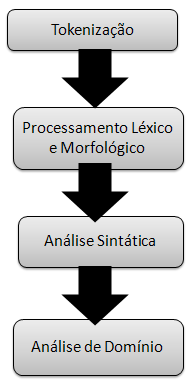
\includegraphics[scale=0.5]{./figuras/EI-estrutura.png}				
				\end{center}
				\caption{Principais m�dulos de um sistema de Extra��o de Informa��o}
                \label{fig:EI-estrutura}
			\end{figure}
			
		Para melhor ilustrar o processo de Extra��o, vamos exemplificar aplicando sobre a senten�a ``O dia � belo'' as quatro etapas do processo.
		 
		Tokeniza��o � a etapa onde dividimos os textos em tokens. Em EI, comumente adota-se a defini��o de um \emph{token} sendo as palavra separadas por espa�o, e.g., na frase ``O dia � belo'', obtemos quatro tokens: ``O'', ``dia'', ``$\acute{e}$'' e ``belo''. Este exemplo ilutra o processo de Tokeniza��o. Em alguns idimas este processo � simples, mas em outros idiomas n�o o �, pela falta de estrutura��o e uma n�o distin��o clara dos limites de uma palavra, e.g., Japon�s, Chin�s.
		
		 O Processamento Morfol�gico e L�xico, adiciona informa��es atrav�s de \emph{tags} classificando l�xica ou morfol�gicamente os \emph{tokens} para posterior utiliza��o, e.g., ``$O_{artigo}$'', ``$dia_{substantivo}$'', ``$\acute{e}_{verbo}$'' e ``$belo_{adjetivo}$''. Neste exemplo, aplicamos regras gram�ticais da l�ngua Portuguesa, mas podemos adotar outras regras como: tamanho da palavra, mai�sculas e minusc�las ou outras criadas a partir do problema a ser resolvido.
		 
		 Muitos sistemas de Extra��o de Informa��o s�o constru�dos sobre a l�ngua inglesa, que n�o necessita uma an�lise morfol�gica muito aprofundada onde uma lista com as varia��es das palavras seria o suficiente. O idioma alem�o por sua vez, � essencial fazer uma an�lise morfol�gica, pois � composto por palavras aglutinadas \cite{Appelt1999}. 
		 
		A maior parte da an�lise do texto � feita atrav�s de um conjunto de express�es regulares \cite{Grishman1997}. A An�lise Sint�tica objetiva estudar a fun��o que as palavras desempenham. Para muitos dom�nios, o simples processo de obten��o de sujeitos, predicados e argumentos resolvem a maioria das senten�as. Se a express�o encontrada estiver inserida no conjunto de express�es regulares, t�o logo ela receber� um marcador, e dependendo do sistema, outros recursos. Com isto dividimos nossa senten�a original em ``$O dia_{Sujeito}$'' e ``$\acute{e} belo_{Predicado}$''.
		 
		 Para demonstrar a An�lise de Dom�nio, tomamos como regra, a obten��o dos substantivos dos sujeitos. Com isto, conseguimos extrair ``dia'' de nossa senten�a original. E finalizamos o processo de extra��o.

		O processo de Extra��o de Informa��o pode ser abstra�do em duas grandes partes. Primeiramente a extra��o \textbf{fatos} individuais do texto atrav�s de uma an�lise textual. Ent�o, a integra��o destes fatos, aumentando os fatos j� obtidos ou criando fatos novos. E por fim, os fatos pertinentes ao cen�rio, n�s transformamos para o formato de sa�da \cite{Grishman1997}. Para isto, o processo passa por algumas complexidades que se relacionam diretamente com os m�dulos que utilizaremos.		
		      
		\paragraph{Fatores de complexidade}	Como a Extra��o de Informa��o trabalha com textos, enfrentamos dificuldades como a l�ngua na qual � escrita, o g�nero do documento, propriedades e a pr�pria tarefa que efetuaremos sobre o documento \cite{Appelt1999}.
		
			\subparagraph{Idioma} Os documentos se encontram escritos em algum idioma, t�o logo nos defrontamos com nossa primeira dificuldade. Algumas l�nguas necessitam de tratamento morfol�gico, espa�amento entre palavras e segmenta��o de palavras. 
			
			\subparagraph{G�nero} O g�nero do documento com o qual se vai trabalhar influ�ncia tamb�m. Se limitarmos nossa ferramenta a textos de an�ncios de jornais, n�o � o mesmo que extrairmos informa��es de artigos cient�ficos. Como consequ�ncia, o uso da linguagem formal ou informal � extremamente ligada ao documento tamb�m.
			
			\subparagraph{Propriedades} Os textos podem conter tabelas, imagens, gr�ficos entre outros tipos de informa��o n�o textual que necessitam de formas especiais de tratamento.
			
			\subparagraph{Tarefas} As tarefas efetuadas pelo sistema tamb�m entram na nossa an�lise de complexidade. Uma ferramenta que apenas procura entidades, possui uma abordagem diferente de uma que procura propriedades a mais de um entidade.
			
		Sistemas de Extra��o de Informa��o trabalham com o processamento de muitos documentos e um espa�o muito curto de tempo. Ent�o, para n�o prejudicar o desempenho, utiliza-se m�quinas de estado finito em abund�ncia. O alvo da extra��o de uma Extra��o de Informa��o pode ser uma rela��o de \emph{n-tuplas} ou muito mais complexa considerando a hierarquia e organiza��o dos dados. 
		
		Programas que realizam a tarefa de Extra��o de Informa��o s�o usualmente chamados de \emph{extratores} ou \emph{wrappers}. Um \emph{wrapper} geralmente executa a tarefa de encontrar padr�es, e estes dependem de um conjunto de regras. Adaptar um sistema de Extra��o de Informa��o tem muitos pontos a serem observados: tipo de texto, dom�nio, cen�rio, conjunto de regras \cite{Chang2006}.
								
		O Reconhecimento de Nomes em um texto � uma tarefa de destaque, uma vez que nomes aparecem frequentemente em todos os tipos de texto, e de muitas maneiras. Os nomes aparecem em um conjunto de padr�o, podendo conter prefixo ou sufixo, estar escrito com letras ma�usculas, facilitando assim sua extra��o. Observando a tabela~\ref{tab:exemplos_nome}, temos algumas maneiras de como o nome Jo�o Jos� da Silva Pereira Junior pode aparecer em um texto.

		% Tabela com exemplos de apari��o de nomes
		\begin{table}[htbp]
		  \centering   
		    \begin{tabular}{rrrr}
		    \addlinespace
		    \toprule
		    {\bf Exemplos de apari��o de nomes} \\
		    \midrule
		    Jo�o Jos� da Silva Pereira Junior \\ 
		    Jo�o Jos� da Silva Pereira Jr. \\
		    Jo�o J. da Silva Pereira Jr. \\
		    Jo�o J. S. P. Jr.\\
		    Sr. Jo�o Pereira Jr. \\
		    JO�O JOS� DA SILVA PEREIRA JUNIOR \\
		    JUNIOR, Jo�o J. S. P.		    
		    \bottomrule
		    \end{tabular}
			\caption{Exemplos de apari��o de nomes}
		  \label{tab:exemplos_nome}
		\end{table}

		Alguns sistemas n�o tem fases distintas para l�xica e sintatica, outros implementam um \emph{parser} para a senten�a inteira. Em geral, os sistemas utilizam partes que possuem certeza sobre sua constru��o, tanto sintaticamente quanto semanticamente. Na analise sint�tica, podemos ainda ter muitas interpreta��es amb�guas, para tal, a sem�ntica e o dom�nio especifico da aplica��o eliminam outras interpreta��es do dados extra�dos.
		
		Construir uma estrutura completa de an�lise sint�tica � extremamente complicada. Algumas decis�es s�o particularmente dif�ceis e dependem do contexto. \emph{Parsers} que buscam avaliar senten�as inteiras pecam no aspecto das decis�es locais, pois procuram ser generalistas para n�o excluirem algumas op��es, acarretando em extrair conte�dos a mais sem muito significado para o dom�nio. Se as rela��es sintaticas forem corretamente extraidas, a interpreta��o dos modelos de cen�rio ser�o mais simples e corretas.

\section{Avalia��o}\label{EI:avaliacao} 
		
		Os crit�rios de avalia��o consistem em: quanta informa��o foi extra�da(\textit{recall}), quanto da informa��o extra�da � correta(\textit{precision}) e quanto da informa��o extra�da � sup�rflua(\textit{overgeneration}) \cite{Sundheim1991}. As confer�ncia \textit{MUC} t�m um papel fundamental na defini��o dessas medidas, na necessidade de avaliar os sistemas de Extra��o de Informa��o. Inicialmente as medidas de precis�o e cobertura foram herdadas do sistema de avalia��o de Recupera��o de Informa��o. Como as t�cnicas de Extra��o e Recupera��o s�o distintas, os nomes foram mantidos, por�m as defini��es das medidas foram alteradas \cite{Gaizauskas1998}.
		 
		\begin{itemize}
          	\item \textbf{Cobertura ou Abrang�ncia}(\textit{Recall}) : Quanto da informa��o extra�da � relevante. Ou seja, � medida atrav�s da informa��o corretamente extra�da($N_{extraido-correto}$) sobre a informa��o relevante na p�gina($N_{total-extraidos}$). Representada pela f�rmula~\ref{formula:cobertura}
          	
          	\begin{equation}\label{formula:cobertura}
              Cobertura = \frac{N_{extraido-correto}}{N_{total-extraidos}}              
            \end{equation}            
    	
          	\item \textbf{Precis�o}(\textit{Precision}) : Quanto da informa��o extra�da � correta. � obtida atrav�s da informa��o corretamente extra�da($N_{extraido-corretos}$) sobre a informa��es extra�das ($N_{resposta}$).
          	
          	\begin{equation}\label{formula:precisao}
              Precis\~{a}o = \frac{N_{extraido-correto}}{N_{resposta}}
            \end{equation}
						
			Importante ressaltar que $N_{total-extraido}$ e $N_{resposta}$ s�o inversamente proporcionais, isto �, quando a \emph{Cobertura} aumenta, a \emph{Precis�o} tende a diminuir e vice-cersa. \emph{Precis�o} e \emph{Cobertura} est�o sempre no intervalo de $[0, 1]$, sendo 0 o pior resultado e 1 o melhor.
			  
  		 	\item \textbf{\textit{F-measure}} : A \textit{F-measure} mede considerando a precis�o e a cobertura. O par�metro $\beta$ controla o balanceamento entre a cobertura e a precis�o. 
  		 	
  		 	\begin{equation}\label{formula:F-measure}
              F-measure = \frac{(\beta^2 + 1)*Cobertura*Precis�o}{\beta^2 * (Cobertura + Precis�o)}
            \end{equation}

			$\beta = Cobertura/Precis\~{a}o$, onde encontramos a F-measure sendo orientada para cobertura quando $\beta > 1$  e orientada para a precis�o quando $\beta < 1$. Por este motivo, geralmente utiliza-se $\beta = 1$ , balanceando assim as duas medidas, e aplicando na f�rmula~\ref{formula:F-measure} temos:

  		 	\begin{equation}\label{formula:F1}
              F_1 = \frac{2*Cobertura*Precis�o}{(Cobertura + Precis�o)}
            \end{equation}			   

        \end{itemize} 

		Para ilustrar melhor os c�lculos, utilizando-se da ferramenta em desenvolvimento pelo autor criada para o projeto \textit{Salus Cyted}, que ser� discutida no capitulo~\ref{Capitulo 5}. A ferramenta \emph{NameParser} ser� aplicada na p�gina \textit{Association Alzheimer\footnote{Association Alzheimer - http://www.alz.org/}}, vista na figura~\ref{fig:siteAssociationAlzheimer} como nossa fonte de dados.

			\begin{figure}[htb]
				\begin{center}				
					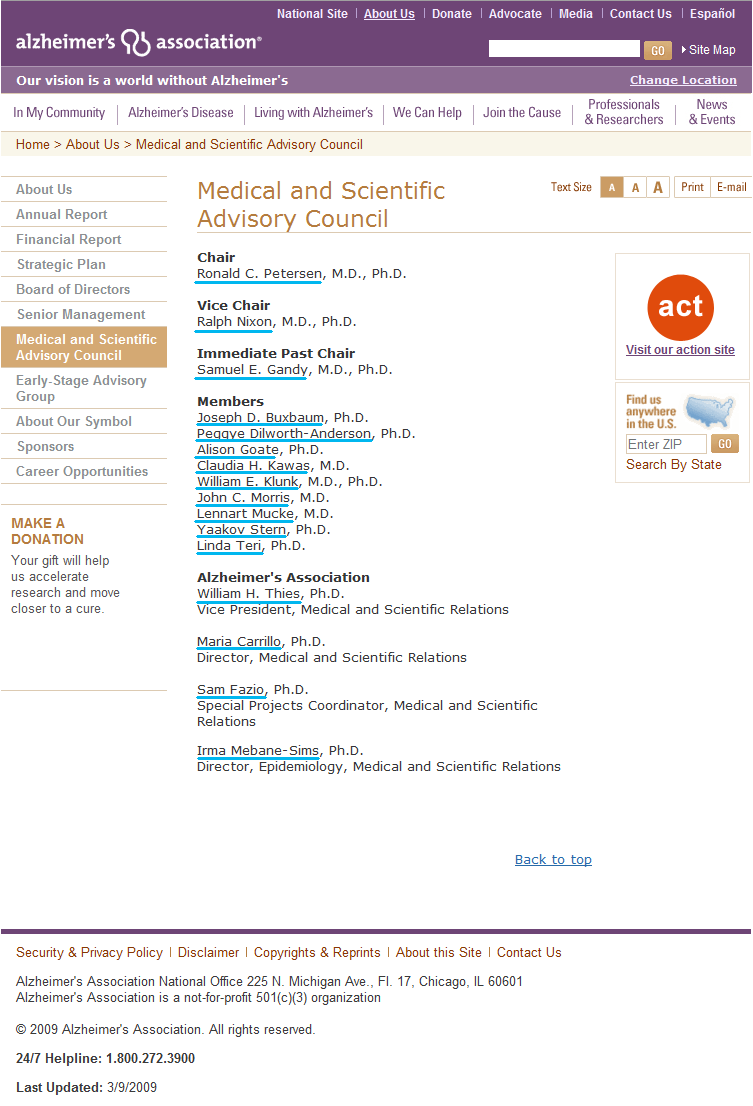
\includegraphics[scale=0.35]{./figuras/site_nome_grifado.png}				
				\end{center}
				\caption{Homepage da Association Alzheimer com nomes extraidos.}
                \label{fig:siteAssociationAlzheimer}
			\end{figure}

		A regra criada para a extra��o de nome tem como base as defini��es da gram�tica, sendo considerado um nome uma palavra que come�a com uma letra mai�scula seguida de letras min�sculas. Como os nomes est�o sendo extra�dos de p�ginas \textit{Web}, e elas n�o possuem uma regra quanto a sua est�tica, podemos encontrar muitas palavras que n�o s�o necessariamente um nome. E isto realmente acontece, como podemos observar na tabela~\ref{tab:termos_extraidos}. 

			\begin{table}[htbp]
              \centering              
                    \begin{tabular}{rrrr}
                        \addlinespace
                        \toprule
                                Termos extra�dos \\
                        \midrule                              
                        		Medical & President & Alzheimer & Scientific \\
                                About & Anual & Report & Plan \\                    
                                Ralph & Nixon & Samuel & Lennart \\
                                Michigan & Chicago & National & Office \\                                                             
                        \bottomrule
                    \end{tabular}
                \caption{Exemplos de alguns termos extraidos}
              \label{tab:termos_extraidos}
            \end{table}
		
		Para esclarecer um pouco mais o conceito de Precis�o e Cobertura, utilizando-se da tabela~\ref{tab:termos_extraidos}, temos o total de 16 termos extra�dos. Desses 16 termos, apenas 4 s�o nomes corretos e esper�vamos no total 8 nomes, ent�o nossa \textbf{Precis�o} � de 50\%. Resultando em uma precis�o m�dia. A \textbf{Cobertura} s�o os nomes extra�dos corretamente sobre o total de termos que extra�mos, resultando em apenas 25\%. Isso significa que de toda informa��o extra�da, apenas 25\% � relevante para o dom�nio do sistema. Note que extraimos nomes como Michigan e Chicago, que est�o corretos do ponto de vista de serem nomes, mas s�o nomes de lugares, e o foco � nome de pessoas.
		
		Temos como resultante a tabela ~\ref{tab:resultados_alzheimerassociation}.
				
            \begin{table}[htbp]
              \centering              
                    \begin{tabular}{rr}
                        \addlinespace
                        \toprule
                              & P�gina \\
                        \midrule                              
                                Nomes presentes & 8 \\
                                Nomes identificados pelo programa (usando express�es) & 16 \\
                                Nomes corretamente identificados (usando express�es) &  4\\
                                Precis�o/Precision & 50\% \\
                                Cobertura/Recall & 25\% \\                              
                        \bottomrule
                    \end{tabular}
                \caption{Resultados da extra��o}
              \label{tab:resultados_alzheimerassociation}
            \end{table}

        O processo de avalia��o � muitas vezes efetuada manualmente ou semi-automatizada. Em algum ponto do processo de avalia��o � necess�ria a interven��o do usu�rio. Para o sistema saber se um dado termo extraido � um nome, o usu�rio que possui esse conhecimento passa de alguma maneira para o sistema.
                        
        Devemos lembrar tamb�m que o dom�nio atribuido ao resultado � muito importante, por exemplo, se encontrarmos um nome pela metade, devemos consider�-lo errado ou correto? Quando o nome se repete ao longo do p�gina, devemos conta-lo apenas uma vez ou mais vezes? Quest�es assim dificultam o crit�rio e devem ser relevadas para uma melhor interpreta��o dos dados.
        
				
		%Extra��o de Informa��o baseada em conhecimento 
		
		%O papel de padr�es ling��sticos � sustentar a interpreta��o de textos na Extra��o de Informa��o baseada em conhecimento. Em fun��o da constru��o de padr�es ling��sticos ser um gargalo mesmo em dom�nios limitados, prop�s-se o uso de um mecanismo de aprendizagem indutivo para construir automaticamente uma base de conhecimento de padr�es. O sistema autom�tico � constru�do sempre que se identifica um padr�o ling��stico desconhecido. Um pressuposto importante embasando esta pesquisa � o reduzido n�mero de express�es normalmente utilizado para descrever uma informa��o dentro de um dom�nio limitado (Kim & Moldovan, 1995).
 
		%Template Mining
		
		%Template Mining ou minera��o por modelos � uma t�cnica de processamento de LN que extrai dados de textos que possuem padr�es que permitam o reconhecimento do que se deseja extrair ou de seus arredores. Um modelo cont�m informa��o sobre o que procurar no texto e � disparado a extrair determinadas partes devidamente indicadas. Lawson et al., (1996) descreve aplica��es de template mining em dom�nios restritos alegando que esta t�cnica � pr�pria para �reas cujos textos s�o claros com frases objetivas e de natureza declarativa.
 
		%Text windowing
		
		%A t�cnica text windowing � do tipo orientada para corpus de textos que avalia palavras na busca de blocos de palavras que estejam relacionadas por sint�tica ou propriedades l�xicas. Jacquemin (1996), descreve uma aplica��o de text windowing em um m�todo para selecionar trechos de textos motivados por propriedades l�xicas, combinando informa��o conceitual em listas de termos com metaregras em filtros sem�nticos locais.
 
		%Documentos Auto-Explicativos
		
		%Consideramos adequado associar a t�cnica de template mining com a metodologia proposta por Branting & Lester (1996) para documentos auto-explicativos. Nesta metodologia, os textos s�o analisados e classificados por sua estrutura ret�rica. A liga��o entre as t�cnicas se d� pelo aproveitamento das estruturas ret�ricas como fonte para a defini��o dos par�metros dos modelos usados pela t�cnica de template mining para extra��o de dados.
 
		%Aquisi��o de Conhecimento de Textos
		
		%O trabalho publicado pelo Grupo de Engenharia de Conhecimentos de Textos da Universidade de Freiburg atrav�s de diversos artigos descreve os esfor�os para analisar textos que apresentam novas formas de conhecimento. O grupo se utiliza de um parser de LN e almeja a expans�o desta base de conhecimento. Da mesma forma que os grupos que tomaram parte dos MUCs, eles tamb�m usam t�cnicas com modelos; entretanto, eles permitem que novos modelos sejam adicionados como resultado da aprendizagem de conceitos (Hahn, & Schnattinger, 1997).

		%O ponto central da pesquisa do grupo trata-se da aquisi��o de conhecimento de textos que ocorre com a aprendizagem de conceitos que alimenta um sistema de compreens�o de linguagem natural. A aprendizagem de conceitos em uma plataforma de compreens�o de linguagem natural � orientada para os recursos atrav�s do uso de um Machine Readable Dictionary MRD e � orientada por contexto. Os autores alegam que inferir o significado das palavras baseando-se em informa��es sobre o contexto � mais confi�vel do que procurar por seu significado em um MRD. A aprendizagem de conceitos � concebida com o desenvolvimento de uma abordagem de aprendizagem de ra�zes simb�licas. Um exemplo de aquisi��o de conceito � descrito em Hahn et al. (1996). O projeto do grupo visa duas aplica��es pr�ticas de aquisi��o de conhecimento de textos da l�ngua alem�: artigos sobre testes de produtos de tecnologia de informa��o (100 documentos com 10^5 palavras) e artigos sobre descobertas m�dicas (120,000 documentos com $$10^7 palavras).

		%O trabalho descrito por Mauldin (1991) usa a compreens�o parcial de textos obtida atrav�s de um parser que realiza text skimming para recupera��o de informa��o conceitual, utilizando um banco de dados de scripts que, por sua vez, � alimentado por um m�todo de aprendizagem e um MRD que aprimora o conhecimento l�xico. A recupera��o de informa��o executada pelo sistema ferret � referida como recupera��o de informa��o conceitual porque ao inv�s de realizar a busca atrav�s do uso de palavras-chave (baseada em palavras) � usado conhecimento sobre os conceitos.

		%Um ponto de vista interessante sobre o problema de aquisi��o de conhecimento de textos � descrito em Futrelle & Zhang (1994) que apresenta t�cnicas de bootstrap que podem descobrir a estrutura de ordem da linguagem natural e definir classes de palavras presentes em corpus de textos. A defini��o de classes de palavras � baseada no princ�pio da substitui��o onde o significado de uma palavra � encontrado pela compara��o dos contextos onde as palavras aparecem e onde elas podem ser substitu�das por outra palavra da mesma classe. 
%    \chapter{\textit{Named Entity Recognition}} \label{capitulo3}
	\chapter{Minera��o de Dados na WEB} \label{capitulo2}

% \section{}
		No inicio, a \textit{Web} continha p�ginas est�ticas objetivando um acesso c�modo as informa��es. Muitas p�ginas eram manualmente implementadas, sem contemplar muito a intera��o com o usu�rio. Geralmente seguiam a dire��o servidor-usu�rio.
		
		Com a expans�o e o acesso crescente, as p�ginas come�aram a evoluir, assim como a \textit{Web}. Tornando-se din�mica, onde encontramos p�ginas constru�das interagindo-se com o usu�rio. Nos encontramos neste est�gio evolutivo, e caminhamos para um futuro muito mais brilhante.
		
		E como a evolu��o n�o tem fim, estamos observando a concep��o da \textit{Web} Sem�ntica. Onde apenas apresentar as informa��es para o usu�rio n�o � o suficiente, como � preciso, expressar de uma forma sem�ntica tamb�m para o entendimento das m�quinas.
		 
		Alguns problemas podem ser encontrados pelos usu�rios quando interagem com a \textit{Web}\cite{Kosala2000}:
  
		 \begin{itemize}
		   \item[a.] \textbf{Achar informa��es relevantes} - Os usu�rios quando utilizam servi�os de pesquisa, procuram atrav�s de palavras-chaves alguma informa��o na \textit{Web}. O resultado da busca, as vezes, � enorme e com isso temos: resultados relevantes, pouco relevantes ou sem relev�ncia;
		   
		   \item[b.] \textbf{Personaliza��o da informa��o} - Usu�rios diferentes, interagem diferentemente e querem conte�dos diferentes, logo, temos o problema no lado do usu�rio e do pr�prio provedor;   
		 \end{itemize}
    
		A \textit{Web Mining} foi concebida devido aos estudos nas mais diversas linhas de pesquisa: extra��o de informa��o, intelig�ncia artificial, banco de dados, recupera��o de informa��o e entre outras �reas. Ela faz parte de um todo, que auxiliam de uma maneira para a resolu��o dos problemas acimas citados.

\section{Web Mining}
	
		\textit{Web Mining} � o uso das t�cnicas de Minera��o de Dados para descobrir e extrair automaticamente a informa��o de documentos na Web\cite{Etzione1996}. A Minera��o de Dados refere-se ao processo n�o trivial de identifica��o de padr�es v�lidos, previamente desconhecidos e potencialmente �teis de dados\cite{Frawley1992}. Seguindo o conceito de Etzione, que utiliza da KDD(\textit{Knowledge Discovery Database}) como base, ele decomp�e a Web Mining em 4(quatro) tarefas:
		 
		\begin{enumerate}
          \item \textit{Resource finding}(Coleta de Documentos);
          \item \textit{Information selection and pre-processing}(Pr�-processamento);
          \item \textit{Generalization}(Extra��o de Padr�es);
          \item \textit{Analysis}(An�lise).
        \end{enumerate}
		
		� importante ressaltar que \emph{Web Mining} � diferente de Recupera��o da Informa��o(\emph{Information Retrieval}) e Extra��o da Informa��o(\emph{Information Extraction}). Mas as t�cnicas s�o utilizadas nas etapas do \emph{Web Mining}.		 
		
		\subsection{Minera��o na WEB de Conte�do}\label{webmining:conteudo} - �udio, v�deo, dados simb�licos, metadados e v�nculos de hipertexto fazem parte do conte�do de documentos da \textit{Web} atualmente, e como tal, na minera��o de conte�dos tamb�m s�o analisados. Existem �reas de pesquisas destinadas a minera��o de dados multim�dias, entretanto, como uma enorme parte da \textit{Web} � constitu�da de texto e hipertexto, portanto o foco permanece em dados de texto. Estes podem ser encontrados em tr�s tipos: desestruturados (textos), semi-estruturados (\textit{HTML}) e estruturados (\textit{XML}).
	 
		A �rea de minera��o de textos est� bem esclarecida, com muitas t�cnicas, uma das quais seria reestruturar o documento para uma linguagem entendida pela maquina. Uma minera��o que vem ganhando destaque em pesquisas � a minera��o em servi�os da Web tais como grupo de noticias, grupos de e-mails, lista de discuss�o. Outro conceito � introduzido por estes pesquisadores, chamado de \textit{Web Intelligence}, que promete transformar os servi�os da \textit{Web} em entidades inteligentes, de forma que elas possam interagir e se comunicar atrav�s de uma linguagem comum. A minera��o de conte�do e a recupera��o de informa��o s�o muitas vezes utilizadas em conjunto. Enquanto uma realiza a minera��o diretamente do conte�do dos documentos a outra incrementa o poder de busca de outras ferramentas e servi�os. 
			
		Duas abordagens s�o utilizadas na minera��o de conte�do, utilizando agentes ou baseadas em banco de dados. As baseadas em banco de dados procura transformar os dados da Web em modelos estruturados para facilitar o trabalho. Utilizando agente, um sistema de intelig�ncia artificial que aja de forma aut�noma ou semi-aut�noma � necess�rio. 

		\subsection{Minera��o de estrutura}\label{webmining:estrutura} - Como o pr�prio nome descreve, nesta categoria de minera��o estamos preocupados com a estrutura dos documentos \textit{Web} e como estes est�o ligados entre si. Os v�nculos de liga��o de hipertexto s�o os principais objetos de estudos nesta categoria. Podemos visualizar a \textit{Web} como um grafo orientado, onde os n�s representam p�ginas e as setas entre os pares de n�s representam os v�nculos entre as paginas. Como ocorre em cita��es bibliogr�ficas quando um artigo � bastante citado indicando que provavelmente este artigo tem um peso importante perante outros que abordam o mesmo tema, o mesmo pode ser observado entre os documentos \textit{Web}. Podemos drasticamente comparar que se uma pagina tem muitas setas entrando, ela teria certa relev�ncia quanto ao seu conte�do ser confi�vel. 

 		\subsection{Minera��o de uso}\label{webmining:uso} - A minera��o de uso utiliza os dados secund�rios provindos de logs de servidores, logs de browsers, perfis de usu�rio, cookies, se��es ou transa��es de usu�rios, pasta favoritos, consultas do usu�rio, cliques de mouse e qualquer outro dado gerado pela intera��o do usu�rio com a \textit{Web}. As aplica��es da minera��o de dados de uso s�o classificadas em duas categorias: aprendizado de perfil de usu�rio (modelagem em interfaces adaptativas) e aprendizado de padr�es de navega��o de usu�rio. Talvez umas das t�cnicas em mais utiliza��o atualmente, devido ao grande n�mero de e-commerce, pois com isto podemos adaptar sites de acordo com o cliente, recomendar produtos de acordo com compras passadas ou baseadas nas similaridades entre perfis de usu�rios. 

        \subsection{Web Semantica}\label{webminig:semantica}

		A minera��o em dados provindos da Web � multidisciplinar, pois muitas �reas s�o utilizadas como: recupera��o de dados, aprendizagem de maquina, agentes de informa��o. Uma �rea muito vasta de interessante pesquisa, e com um futuro muito promissor, pois dia ap�s dia vemos a Web crescer e por enquanto, seu horizonte parece n�o ter fim. 
	\chapter{Caso de Uso - Projeto Salus Cyted}\label{Capitulo 5}

		O projeto Salus Cyted nasceu com o objetivo de estimular a participa��o coletiva e estruturar uma s�lida coopera��o entre os grupos participantes, e para tanto, as atividades foram centralizadas em um ambiente espec�fico: um Portal Web com acesso adapt�vel aos diferentes usu�rios em fun��o de seu n�vel cultural e peculiaridades regionais.
	
\section{Cria��o do Parser}
	
		\textbf{Parser} - � um componente de um programa que analisa a estrutura l�xica de uma entrada de acordo com regras pr�-definidas. E para a cria��o do 
	
		A ferramenta para a implementa��o do NameParser foi o JavaCC(Java Compiler Compiler[tm]). � um gerador de parser \textit{open-source} inicialmente desenvolvido pela \textit{Sun}. Utiliza uma sintaxe pr�xima do Java, e trabalha \textit{top-down}.
	 
		Um Parser � um programa de computador (ou apenas um componente de um programa) que serve para analisar a estrutura gramatical de uma entrada, manipulando os tokens, que s�o segmentos de texto ou s�mbolos que podem ser manipulados. Em XML, o parser pode ser um leitor que ajuda na convers�o do arquivo para manipula��o dos dados contidos no mesmo.
	
		A cria��o do Parser para a extra��o de nomes em paginas, foi desenvolvida em v�rias etapas. No primeiro momento, foi criado a Express�o Regular para a extra��o de nomes. A Express�o foi concebida analisando como os nomes aparecem em nossa escrita. Por exemplo: Pedro de Alc�ntara Francisco Ant�nio, podemos encontrar ele escrito nas seguintes formas: Pedro de A. F. Antonio, Pedro A. F. Ant�nio, Pedro de A. Francisco Ant�nio. Ainda temos que relevar se ele publicou algum artigo ou outro documento do g�nero, onde segue-se uma regra espec�fica, logo, podemos encontrar o nome escrito nas seguintes formas: "de A. F. A, Pedro.", 
 
	\renewcommand{\baselinestretch}{0.5}  % dist�ncia entre linhas
	\begin{codigo}[htb]
	   \tiny  % tamanho da fonte
	   \begin{boxit}  % coloca o c�digo dentro de um Box
	      \vspace{2mm}
	      \VerbatimInput[xleftmargin=8mm,numbers=left,obeytabs=true]{./codigos/Teste.java}
	   \end{boxit}
	   \caption{\it C�digo de teste Java }
	   \label{code:Teste}
	\end{codigo}
		
%	\chapter{Conclus�o}

		At� o momento, � apresentado um conceito b�sico sobre Recupera��o de Informa��o, para podermos prosseguir para a Extra��o de Informa��o. Os conceitos de Extra��o de Informa��o s�o abordados mais profundamente, porque a tecnica que buscamos enfatizar se encontra neste capitulo. Ent�o, entramos no assunto de Minera��o de Dados na Web para finalizar uma vis�o geral das Tecnicas de Extra��o de Dados na WEB.
		
		Em rela��o ao cronograma, estou pesquisando e lendo algumas literaturas mais atuais sobre os assuntos de Web Mining, com um enfoque especial em Web Sem�ntica e em Extra��o de Informa��o, a pesquisa em Reconhecimento de Entidades Mencionadas(\emph{Named Entity Recognition}).
		
		Um capitulo ser� abordado tamb�m sobre um estudo de caso, mantendo o foco em Reconhecimento de Entidades Mencionadas, que � uma ferramenta que analisaremos particularmente e faz parte de um projeto muito maior. Como pode-se observar, o capitulo da ferramenta tem apenas uma descri��o breve de seu funcionamento. 				
	
	\bibliographystyle{abnt-alf}
	\bibliography{./bibliografia/bibliografia}

\end{document}
